The backend is designed based on the three-layer spring architecture, which is dividing the code base into three separated layers of abstraction, which help in isolating components in the codebase and facilitate SOLID and clean code principles. 

The upper layer is where the controllers live and manage client requests. The business logic layer contains the needed services in which we apply any logic needed for managing the application. The last layer consists of the repositories which communicate with the database using ORM supported by Hibernate. The three layered architecture can be seen in Figure \ref{fig:threelayerArch}
\\
\begin{figure}[h]
    \centering
    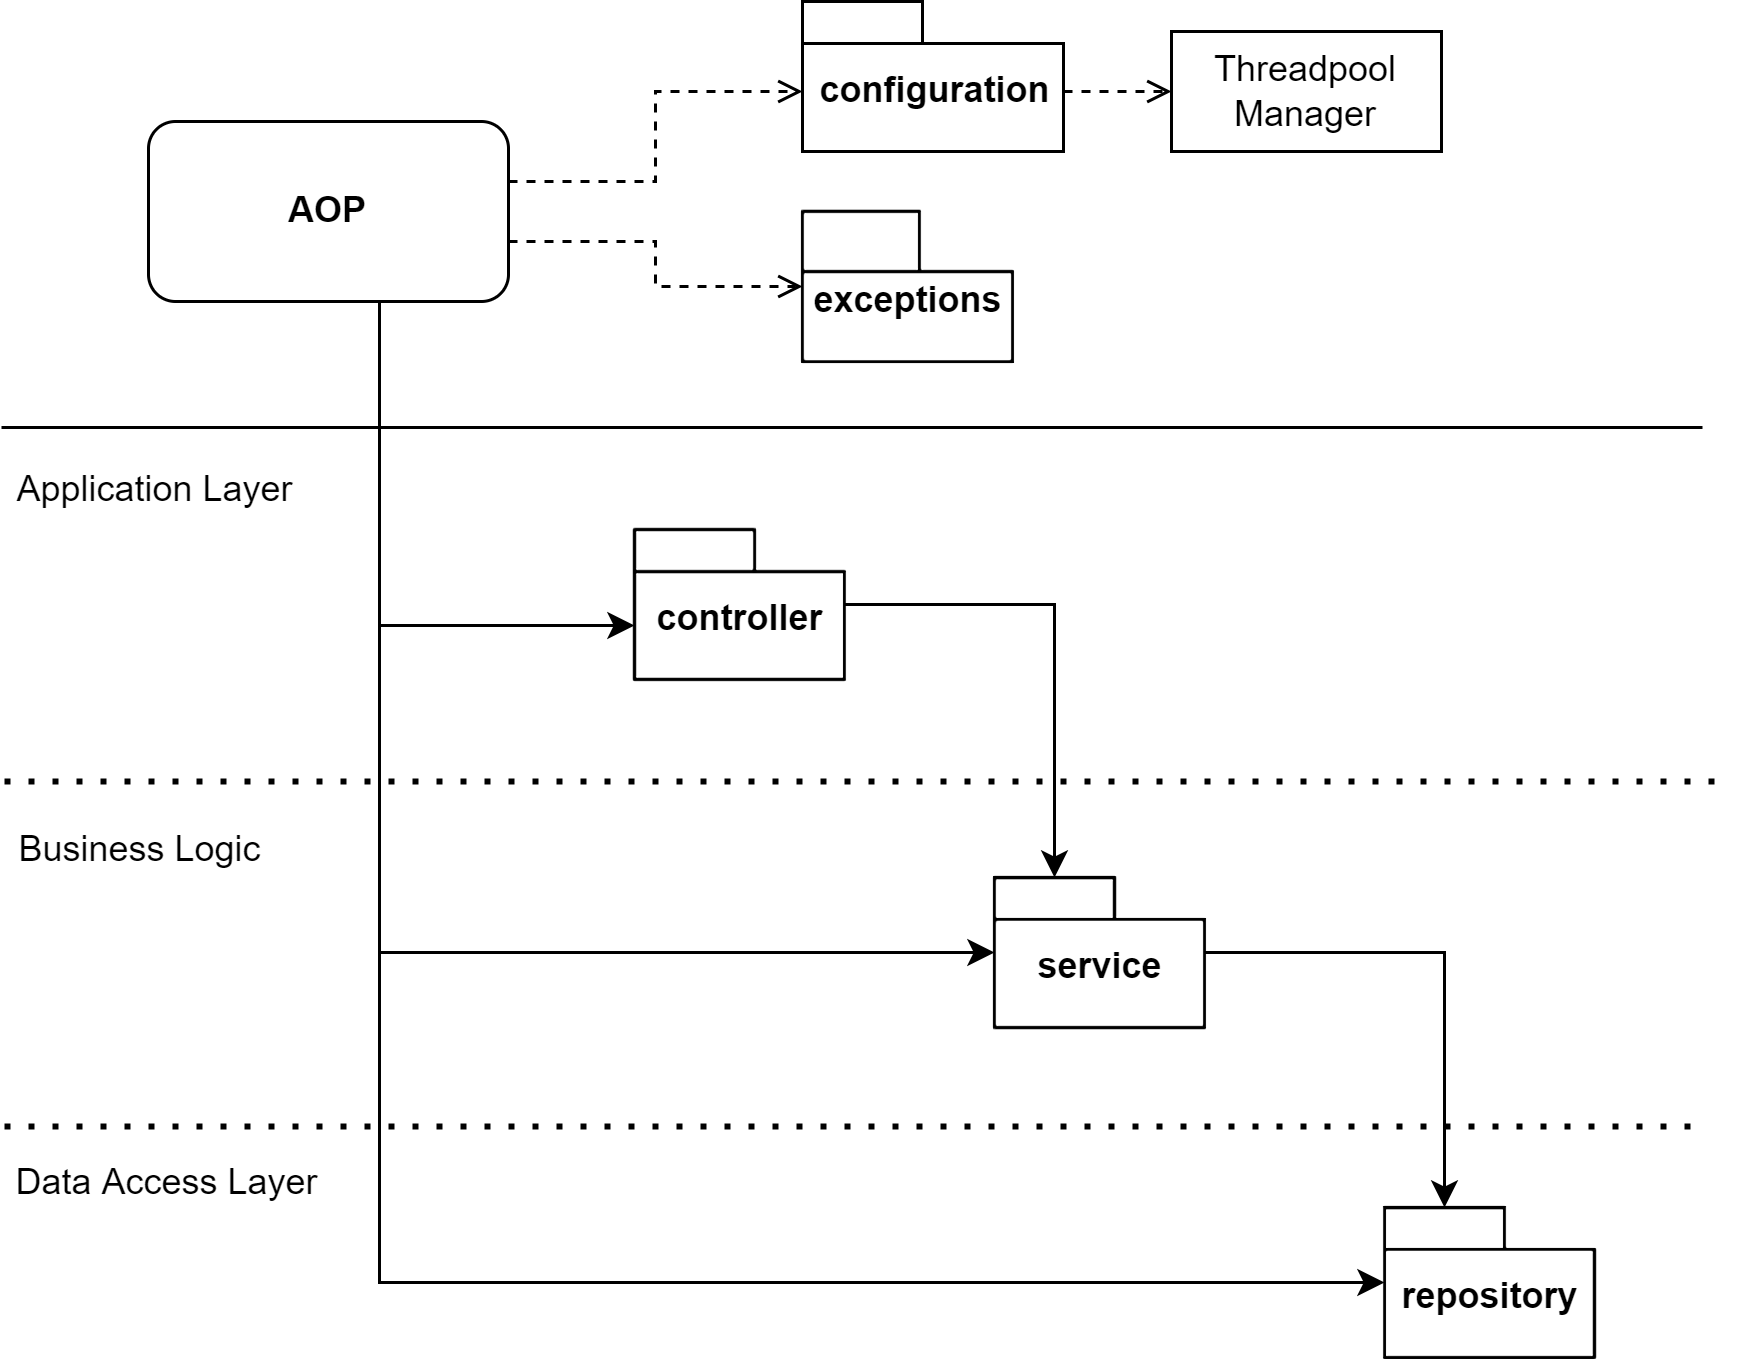
\includegraphics[width = .9\textwidth]{images/ThreeLayerArchitecture.png}
    \caption{Three layered architecture shown in package diagram}
    \label{fig:threelayerArch}
\end{figure}\\

The layers are connected using the dependency injection container to ensure that the code is loosely coupled, and all the dependencies are loaded to each component during the initialization phase of the server. Exception handling and other configuration, e.g., thread pool management and database configuration context load are handled using aspect-oriented programming and proxy pattern which clean the code from all the boilerplates try-catch blocks and NPE.
\newpage
\subsubsection{Simplified 3+1 architecture}
For this project, use a simplified 3+1 architecture, in this regard we looked at the module viewpoint with a package diagram of the backend as well as an allocation viewpoint via a deployment diagram.\\
The concern of a module viewpoint is to look at how the functionality of the code is organized. For this we refer back to Figure \ref{fig:threelayerArch} which shows a package diagram where the packages are separated into different layers to account for the three layered architecture of our system.\\
For the allocation viewpoint, a simple deployment diagram was created - this diagram shows how all three elements within the system are connected to the same VM, the element backend is then connected to the database. See Figure \ref{fig:deploymentDiagram}
\begin{figure}[h]
    \centering
    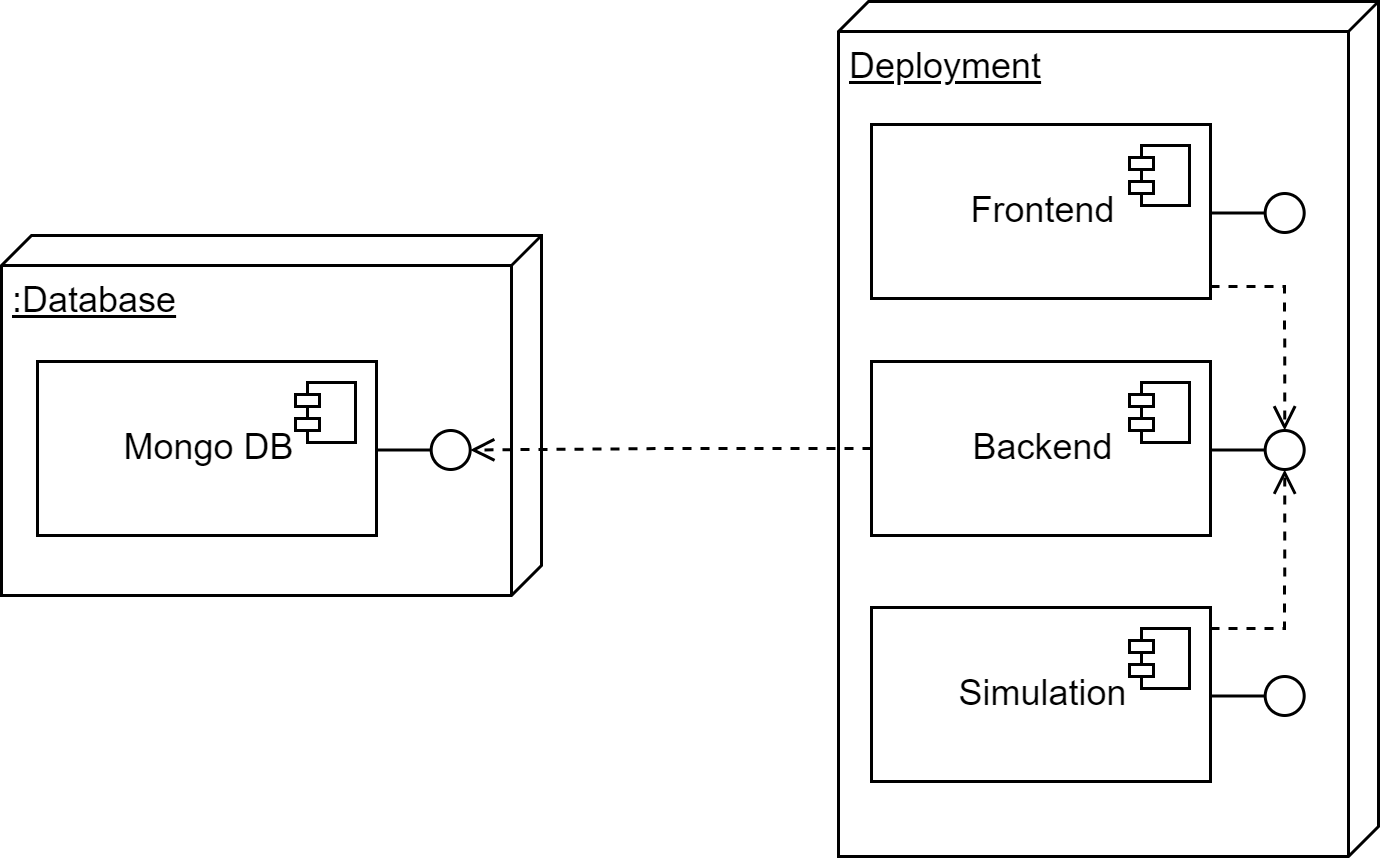
\includegraphics[width =.7 \textwidth]{images/DeploymentDiagram.png}
    \caption{Deployment diagram of the system}
    \label{fig:deploymentDiagram}
\end{figure}
